%Template retirado da página do DI.
\documentclass{report}
\usepackage{graphicx}
\usepackage[portuguese]{babel}
\usepackage[utf8]{inputenc}
\usepackage{hyperref}
%\usepackage[latin1]{inputenc}
%\usepackage{url}
\usepackage{color}
\usepackage{enumerate}
\usepackage{alltt}
\usepackage{fancyvrb}
\usepackage{listings}
\usepackage{amsmath}
\usepackage{verbatim}
\usepackage{xcolor}
\usepackage{listings}

\lstset{breaklines=true}
\DefineVerbatimEnvironment{code}{Verbatim}{fontsize=\footnotesize}
%LISTING - GENERAL
\lstset{
	basicstyle=\small,
	numbers=left,
	numberstyle=\tiny,
	numbersep=5pt,
	breaklines=true,
    frame=tB,
	mathescape=true,
	escapeinside={(*@}{@*)}
	}

\usepackage{xspace}

\parindent=0pt
\parskip=2pt

\setlength{\oddsidemargin}{-1cm}
\setlength{\textwidth}{18cm}
\setlength{\headsep}{-1cm}
\setlength{\textheight}{23cm}

\def\darius{\textsf{Darius}\xspace}
\def\antlr{\texttt{AnTLR}\xspace}
\def\pe{\emph{Publicação Eletrónica}\xspace}

\def\titulo#1{\section{#1}}
\def\super#1{{\em Supervisor: #1}\\ }
\def\area#1{{\em \'{A}rea: #1}\\[0.2cm]}
\def\resumo{\underline{Resumo}:\\ }


\title{Processamento de Linguagens e Compiladores (3º ano de LCC/4º ano de MIEFis)\\ \textbf{Compilador de uma Linguagem Imperativa}}
\author{Jaime Santos (A71739) \and Hugo Sousa (A76257) \and Luís Bigas (A76964) }
\date{\today}

\begin{document}

\maketitle

\begin{abstract}
Neste relatório irá ser analisada a implementação, e os desafios associados, de um compilador de uma linguagem imperativa original através do uso do conjunto de ferramentas \textit{Yacc} e \textit{Flex}. \\
\end{abstract}

\tableofcontents

\chapter{Introdução}
Para este trabalho pretende-se demonstrar os conhecimentos adquiridos pelo grupo na aplicação de GIC's(Gramáticas Independentes de Contexto).\\
Para tal, tem-se como objetivo a criação de um compilador, para uma simples linguagem de programação imperativa, constituído pelo analisador sintático em \textit{Flex} que irá reconhecer e devolver os simbolos terminais como tokens ao analisador léxico em \textit{Yacc}. O \textit{Yacc} irá então avaliar a validade das frases fornecidas e executar uma dada ação, como a geração de erros de compilação e código Assembly para a VM.
\section{Estrutura do Relatório} 
No seguinte capitulo, irão ser analisados os requisitos para a resolução do trabalho proposto pelo professor, que se baseiam nas capacidades que a linguagem criada terá que apresentar.\\
No capitulo 3 apresenta-se primeiramente uma visão geral da implementação da solução para este trabalho, seguida da especificação em detalhe desta solução.\\
No capitulo 4 demonstra-se o funcionamento da linguagem criada através do uso de exemplos de código e o respetivo output na VM fornecida pelo professor seguido de uma breve reflexão dos resultados obtidos.\\
No 5º e ultimo capitulo encontra-se a conclusão, onde irão ser discutidas as limitações da implementação, desafios encontrados e uma perspetiva geral da linguagem criada. \\


\chapter{Objetivo do Trabalho}
Na criação deste compilador de uma linguagem imperativa, temos como objetivo a criação de uma Gramática Independente de Contexto com as seguintes capacidades:
\begin{enumerate}
\item Declaração de variáveis de tipo Inteiro, Real e Booleano.
\item Atribuição de valores a variáveis.
\item Capacidade de execução de operações aritméticas e comparação.
\item Execução de condições (\textit{IF THEN ELSE}) e ciclos (\textit{REPETIR...ATÉ})
\item Escrita de Inteiros, Reais, Booleanos e \textit{Strings}.
\item Leitura de input (Inteiros e Reais) por parte do utilizador.
\end{enumerate}
Para além dos requisitos minimos, foi decidido implementar as seguintes funcionalidades:
\begin{enumerate}
\item Incrementar e Decrementar uma variável Inteira.
\item Calcular o seno e cosseno de uma variável Real.
\item Escrita da concatenação de duas \textit{Strings}.
\end{enumerate}
Após estes requisitos serem cumpridos, é necessário verificar o funcionamento da linguagem fornecendo códigos exemplo ao executável que irá imprimir, para um ficheiro do tipo \textit{vm}, as instruções necessárias para o correto funcionamento deste na Máquina Virutal. Estes códigos encontram-se no capitulo 4.

\chapter{Resolução}
Para atingir os objetivos pretendidos neste trabalho, foi realizado em três partes que em conjunto realizam a compilação de uma linguagem imperativa:
\begin{enumerate}
\item A gramática independente de contexto e as suas ações em Bison.
\item Gerador léxico para o reconhecimento do programa a compilar em Flex.
\item Uma biblioteca sobre uma estrutura de dados na linguagem C, criada pelo grupo para facilitar a interpretação e processamento de dados do programa. Esta estrututra irá permitir a indexação de variáveis de modo a impedir que existam multiplas declarações da mesma, bem como a utilização de uma variável nunca declarada.
\end{enumerate}
A Gramática interpreta o padrão do código da linguagem criada, através do gerador léxico, e gera o código assembly lido pela máquina virtual, assim como tratamento de erros.\\
Graças à flexibilidade das ferramentas, o programa Bison utiliza a biblioteca C para complementar a interpretação dos dados recebidos.\\
No próximo capitulo procedemos à demonstração e análise do nosso trabalho.\\
O código utilizado nestas três ferramentas encontra-se em anexo.
\section{Análise e Especificação}
\subsection{Bison/Yacc} 
\subsubsection{Gramática}
\begin{enumerate}
\item A gramática tem inicio com o padrão:\\
\colorbox{lightgray}{Program : START Tasks END}\\
A palavra \textbf{START} indica o inicio do código do programa, a palavra \textbf{END} indica o seu final.

\item Tasks:\\
\colorbox{lightgray}{Tasks : Tasks Task ';'}\\
\colorbox{lightgray}{Tasks :  Task ';'}\\
\textbf{Task} define cada uma das linhas/instruções do programa principal, cada uma das linhas termina com o símbolo terminal ponto e virgula  ";".\\
\textbf{Tasks} é a chamada recursiva do padrão, de modo a que seja possivel reconhecer mais do que uma \textbf{Task}.\\
\\
\\
\\
\\

\item Task:\\
\colorbox{lightgray}{Task : startVars}\\
\colorbox{lightgray}{Task : Inst}\\
\textbf{startVars}: contém as produções necessárias à inicialização de variáveis.\\
\textbf{Inst}:																																																																																																											 representa a derivação que permitirá fazer as restantes ações disponiveis na linguagem.\\
Optou-se por esta estrutura de modo a que seja possivel declarar variáveis e executar ações intercaladamente.

\item startVars:\\
\colorbox{lightgray}{startVars : INT Var}\\
\colorbox{lightgray}{startVars : REAL Var}\\
\colorbox{lightgray}{startVars : REAL Var2}\\
\colorbox{lightgray}{startVars : BOOL Var}\\
\textbf{Var}: Nome da Variável(inteiros e bools)\\
\textbf{Var2}: Nome da Variável(floats)\\
É de notar que, devido à natureza das produções criadas, estas duas derivações foram a estratégia encontrada pelo grupo de modo conseguir distinguir entre variáveis inteiras e reais, sendo esta uma das limitações do trabalho, visto que \textbf{Var} e \textbf{Var2} irão derivar em dois simbolos terminais diferentes de modo a evitar conflitos.\\
\textbf{INT, REAL, BOOL}: Símbolos terminais que determinam o tipo da variável a definir.\\

\item{Var}:\\
\colorbox{lightgray}{Var : STR}\\
\textbf{STR}: Símbolo terminal de reconhecimento do nome de uma variável.

\item{Var2}:\\
\colorbox{lightgray}{Var2 : nome}\\
\textbf{nome}: Símbolo terminal de reconhecimento do nome de uma variável float.

\item{Insts}:\\
\colorbox{lightgray}{Inst : READ Var}\\
\colorbox{lightgray}{Inst : READ Var2}\\
\colorbox{lightgray}{Inst : WRITE Var}\\
\colorbox{lightgray}{Inst : WRITE Var2}\\
\colorbox{lightgray}{Inst : WRITE STRING}\\
\colorbox{lightgray}{Inst : Var INC}\\
\colorbox{lightgray}{Inst : Var DEC}\\
\colorbox{lightgray}{Inst : IF '(' Cond ')' THEN '{' Tasks '}' ELSES}\\
\colorbox{lightgray}{Inst : UNTIL '('Cond')' DO '{'Tasks'}'}\\
\colorbox{lightgray}{Insts : Atrib}\\
\textbf{READ}: Leitura de input do utilizador a partir do standard input.\\
\textbf{WRITE}: Escrita do valor de uma variável no standard output\\
Note-se que tanto no READ como no WRITE, a derivação escolhida irá depender do tipo da variável.\\
Caso esta seja um Inteiro ou Booleano, irá derivar pela \textbf{Var}, caso seja um Real, derivará por \textbf{Var2}, e caso seja pretendido escrever uma String, a derivação escolhida será a da \textbf{STRING}.\\
\textbf{INC, DEC}: Incremento/decremento do valor de uma variável inteira por 1.\\
\textbf{IF '(' Cond ')' THEN '{' Tasks '}' ELSES} Reconhecimento de uma condição if(), else(). \textbf{COND} representa a condição que, se aceite, é executado o código contido entre as chavetas, que irá derivar em \textbf{Tasks}. \textbf{ELSES} reconhece a alternativa de execução quando falha a condição if(), e é nao terminal de modo a ser possível derivar em vazio.\\
\textbf{UNTIL '('Cond')' DO '{'Tasks'}'}: Ciclo REPETIR...ATÈ, que enquanto a condição presente em \textbf{Cond} é falsa, repete o código entre chavetas que deriva em \textbf{Tasks}.\\
\textbf{Atrib}: Define que uma instrução irá poder derivar numa atribuíção, que irá ser descrita de seguida.

\item{STRINGS}:\\
\colorbox{lightgray}{STRINGS : STRING STRINGS}\\
Derivação utilizada quando é pretendido fazer a escrita de Strings, podendo esta ser vazia, ou várias strings delimitadas por " ", que irão ser concatenadas pela Máquina Virtual.

\item{ELSES}:\\
\colorbox{lightgray}{ELSES : \&}\\
\colorbox{lightgray}{ELSES : ELSE '\{' Tasks '\}'}\\
\textbf{\&}: Reconhecimento de uma produção vazia caso não seja utilizada a condição else.\\
\textbf{ELSE '\{' Tasks '\}'}: Reconhecimento do padrão \textbf{ELSE} e execução do código contido nas chavetas que deriva em \textbf{Tasks}.

\item{Atribuições}:\\
\colorbox{lightgray}{Atrib : Var '=' Calc}\\
\colorbox{lightgray}{Atrib : Var2 '=' Calc2}\\
Caso seja derivada uma variável Inteira ou Booleana, a atribuição feita a esta será feita através de \textbf{Calc}. Caso seja um Real, a atribuição será por \textbf{Calc2}.\\

\item{Condições}:\\
\colorbox{lightgray}{Cond : Calc EQ Calc}\\
\colorbox{lightgray}{Cond : Calc NE Calc}\\
\colorbox{lightgray}{Cond : Calc LT Calc}\\
\colorbox{lightgray}{Cond : Calc LE Calc}\\
\colorbox{lightgray}{Cond : Calc GT Calc}\\
\colorbox{lightgray}{Cond : Calc GE Calc}\\
\colorbox{lightgray}{Cond : Calc2 EQ Calc2}\\
\colorbox{lightgray}{Cond : Calc2 NE Calc2}\\
\colorbox{lightgray}{Cond : Calc2 LT Calc2}\\
\colorbox{lightgray}{Cond : Calc2 LE Calc2}\\
\colorbox{lightgray}{Cond : Calc2 GT Calc2}\\
\colorbox{lightgray}{Cond : Calc2 GE Calc2}\\
\textbf{Cond}: Reconhece a comparação entre duas operações aritméticas derivadas ou por \textbf{Calc} ou \textbf{Calc2}.\\
\textbf{EQ, NE, LT, LE, GT, GE}: Representam as noções de Igualdade(==), Diferença(!=), Menor(\textless), Menor ou igual(\textless =), Maior(\textgreater), Maior ou igual(\textgreater =), respetivamente.
\\
\\
\\
\\
\\
\\
\\
\\
\\
\\
\\
\\
\\
\\
\\
\\
\\

\item{Operações Aritméticas}\\
Através das derivações a seguir definidas podemos realizar operações aritméticas básicas.\\
\colorbox{lightgray}{Calc : Exp}\\
\colorbox{lightgray}{Calc : Calc '+' Exp}\\
\colorbox {lightgray}{Calc : Calc '-' Exp}\\

\colorbox{lightgray}{Exp : Fat}\\
\colorbox{lightgray}{Exp : Exp '*' Fat}\\
\colorbox{lightgray}{Exp : Exp '/' Fat}\\
\colorbox{lightgray}{Exp : Exp '\%' Fat}\\

\colorbox{lightgray}{Fat : '(' Calc ')'}\\
\colorbox{lightgray}{Fat : cos '(' Calc ')'}\\
\colorbox{lightgray}{Fat : sin '(' Calc '='}\\
\colorbox{lightgray}{Fat : typeVar}\\
\textbf{Calc '+' ou '-' Exp}: Definição das somas e subtrações de modo a que sejam as ultimas operações aritméticas a ser feitas (caso não existam parênteses).\\
\textbf{Exp}: Derivação que irá reconhecer operações como multiplicação, divisão e módulo (no caso dos Inteiros).\\
\textbf{Fat}: faz o reconhecimento de operações com parênteses e as funções da máquina virtual \textbf{cos e sin}. Irá também receber o valor das variáveis derivadas por \textbf{typeVar}.\\
Desta forma as operações respeitam a prioridade das operações aritméticas, uma vez que o reconhecimento é feito \textit{Bottom Up}.\\\\
\textbf{\underline{MUITO IMPORTANTE}}\\
Todas as operações aritméticas derivadas por \textbf{Calc} são feitas sobre inteiros. Para a diferenciação dos Reais, optou-se por fazer a derivação \textbf{Calc2} que irá ser omitida desta explicação, uma vez que tem uma estrutura semelhante à supracitada, à exceção da operação módulo. Para reconhecimento da variável Real, \textbf{Fat2} irá ter uma produção em \textbf{typeVar2} que contém informação sobre os Reais.


\item{typeVar}\\
\colorbox{lightgray}{typeVar : num}\\
\colorbox{lightgray}{typeVar : rial}\\
\colorbox{lightgray}{typeVar : booleans}\\
\colorbox{lightgray}{typeVar : Var}\\
\textbf{num, booleans}: Reconhecimento literal de um valor Inteiro ou Booleano (simbolo terminal).\\
\textbf{Var}: Usada para atribuir o valor de uma variável Inteira ou Booleana já definida a outra variável Inteira ou Booleana.\\

\item{typeVar2}\\
\textbf{rial}: Reconhecimento literal de um valor Real (simbolo terminal).\\
\textbf{Var2}: Usada para atribuir o valor de uma variável Real já definida a outra variável Real.\\
\end{enumerate}


\section{Flex}
A ferramenta Flex faz a análise léxica para possibilitar o reconhecimento da gramática.\\
Cada uma das instruções do programa Flex faz com que cada um dos símbolos terminais seja reconhecido pela gramática.\\
Por exemplo:\\
\colorbox{lightgray}{"START:"\ \ \ \ \{\  return START;\	\}  }

Reconhece o padrão literal "START:"\ e retorna-o para ser interpretado pela gramática definida no Bison.\\
\colorbox{lightgray}{[a-zA-Z]+\ \ \ \ \{ yylval.terms=strdup(yytext); return STR;\ \}}\\
Reconhece strings, e é copiado o seu conteúdo para a estrutura yylval.

\section{Biblioteca C}
\subsection{Estrutura de dados}
typedef struct pos\{\\
	char* nome;\\
	char estado;\\
    char* type;\\
\}POS[MAX];
\\
\\
\textbf{nome:} uma string com o nome da variável.\\
\textbf{estado:} estado na posição da estrutura de dados(livre ou ocupado).\\
\textbf{type:} tipo de dados guardado em cada uma das posições da estrutura.\\
\subsection{Funções}
\begin{enumerate}
\item \colorbox{lightgray}{void \_initVars ( POS p );}\\
Inicia todas as posições como vazias.
\item \colorbox{lightgray}{int \_isDeclared ( POS p , char* nome );}\\
Verifica se uma variável "nome" existe na estrutura de dados, retorna 0 caso não exista e 1 caso contrário.
\item \colorbox{lightgray}{int \_getposi ( POS p, char *nome );}\\
Retorna a posição da variável(nome) na estrutura que é também a posição desta na stack da máquina virtual.
\item \colorbox{lightgray}{void \_addVar ( POS p, char* nome, char* tipo );}\\
Adiciona uma variável na estrutura.
\item \colorbox{lightgray}{char* \_getType ( POS p, char* nome );}\\
Retorna o tipo da variável(nome).

\end{enumerate}

\chapter{Exemplos de Execução}
Neste capitulo seguem os vários exemplos da execução de códigos, que variam de simples somas e atribuições, a códigos com condições \textit{IF THEN ELSE} com ciclos. Tambem serão testados os erros de multiplas declarações de variáveis e a atribuição a variáveis nunca declaradas.

\section{Soma de inteiros}
Neste exemplo vamos testar a declaração e a soma de dois inteiros. Declaramos o inteiro "a" e escrevemos o valor dele, delcaramos o inteiro "b" e atribuimos a "b" a soma dos dois inteiros imprimimos o resultado.
\subsection{Input:}
\VerbatimInput{1INT.txt}
Podemos ver que o código foi compilado com sucesso e os valores foram gravados nas posições pretendidas.
\subsection{Output:}

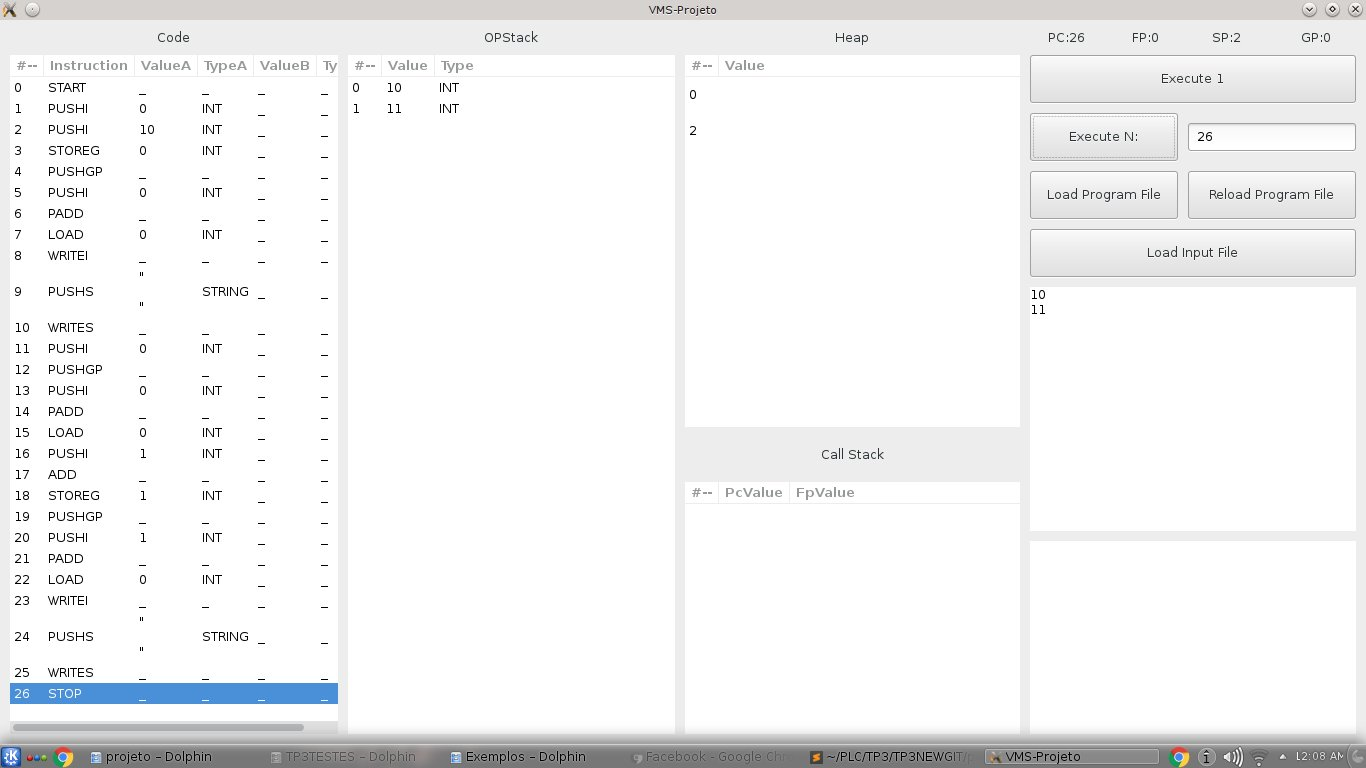
\includegraphics[width=\linewidth]{BasicINT.jpg}

\section{Soma de Floats}
Neste exemplo à semelhança do que tinhamos no exemplo anterior fazemos a declaração, soma e escrita das variáveis mas neste caso em vez de inteiros estamos a usar reais.
\subsection{Input:}
\VerbatimInput{1FLOAT.txt}
Podemos ver que o código foi compilado com sucesso e os valores foram gravados nas posições pretendidas.
\subsection{Output:}

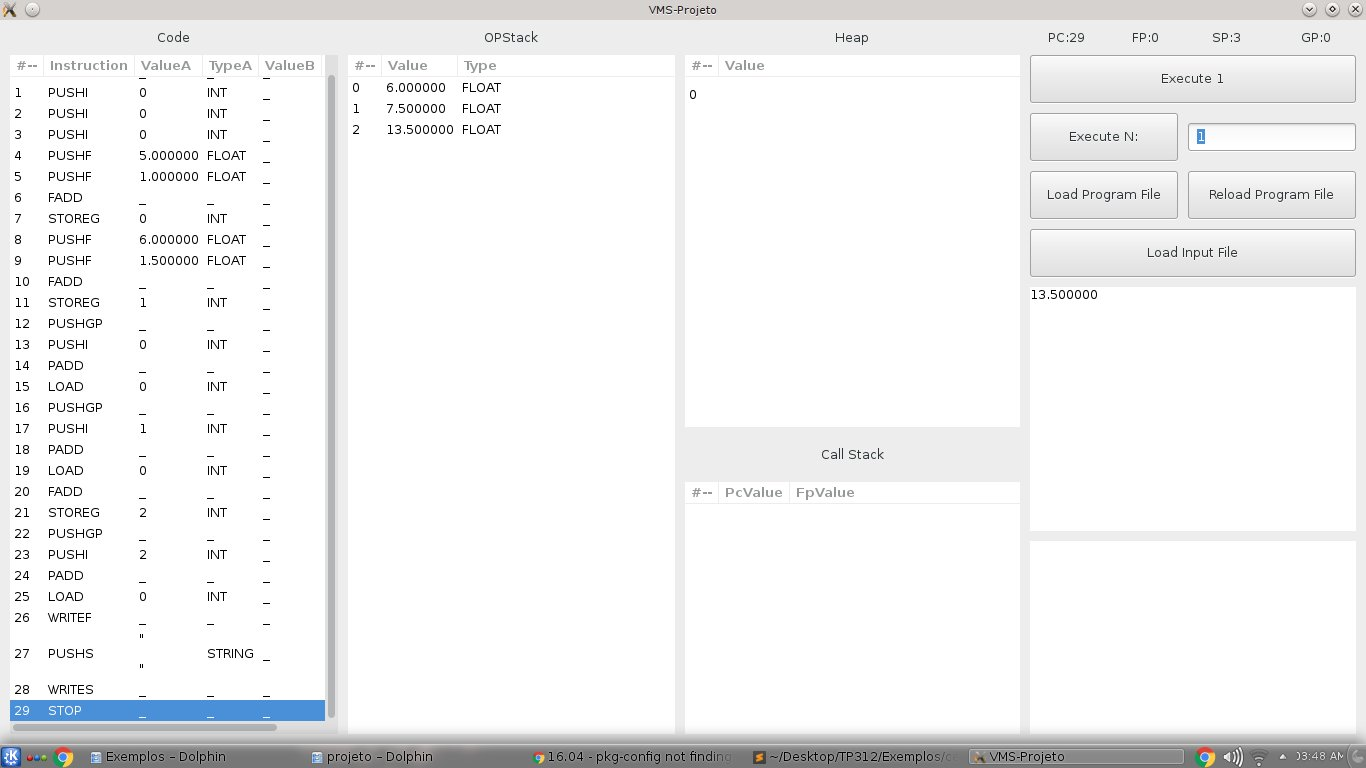
\includegraphics[width=\linewidth]{BasicFLOAT.jpg}

\section{Variável não declarada}
Vamos agora testar detecções de erro, declaramos um inteiro "b" e atribuimos a uma variável não declarada "a" o valor de b.
\subsection{Input:}
\VerbatimInput{1NAODECLARADA.txt}
A mensagem de erro "Variável não declarada" foi escrita corretamente no momento de compilação.
\subsection{Output:}

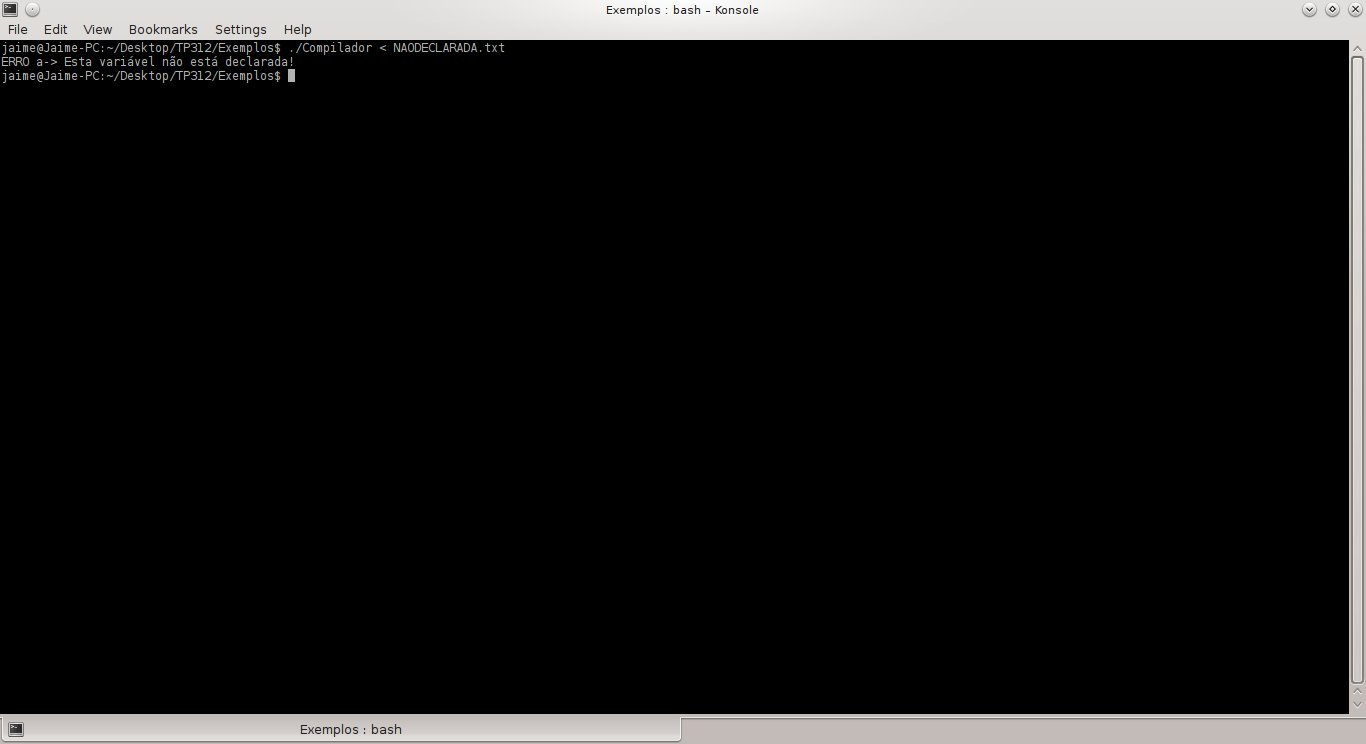
\includegraphics[width=\linewidth]{NaoDeclarada.jpg}

\section{Variável já declarada}
Neste exemplo vamos testar outra detecção de erro, neste caso a redeclaração de variáveis, primeiro declaramos um inteiro "a" e de seguida um booleano também chamado "a".
\subsection{Input:}
\VerbatimInput{1REDECLARADA.txt}
Podemos ver que a mensagem de erro foi escrita no momento de compilação com a mensagem de erro adequada.
\subsection{Output:}

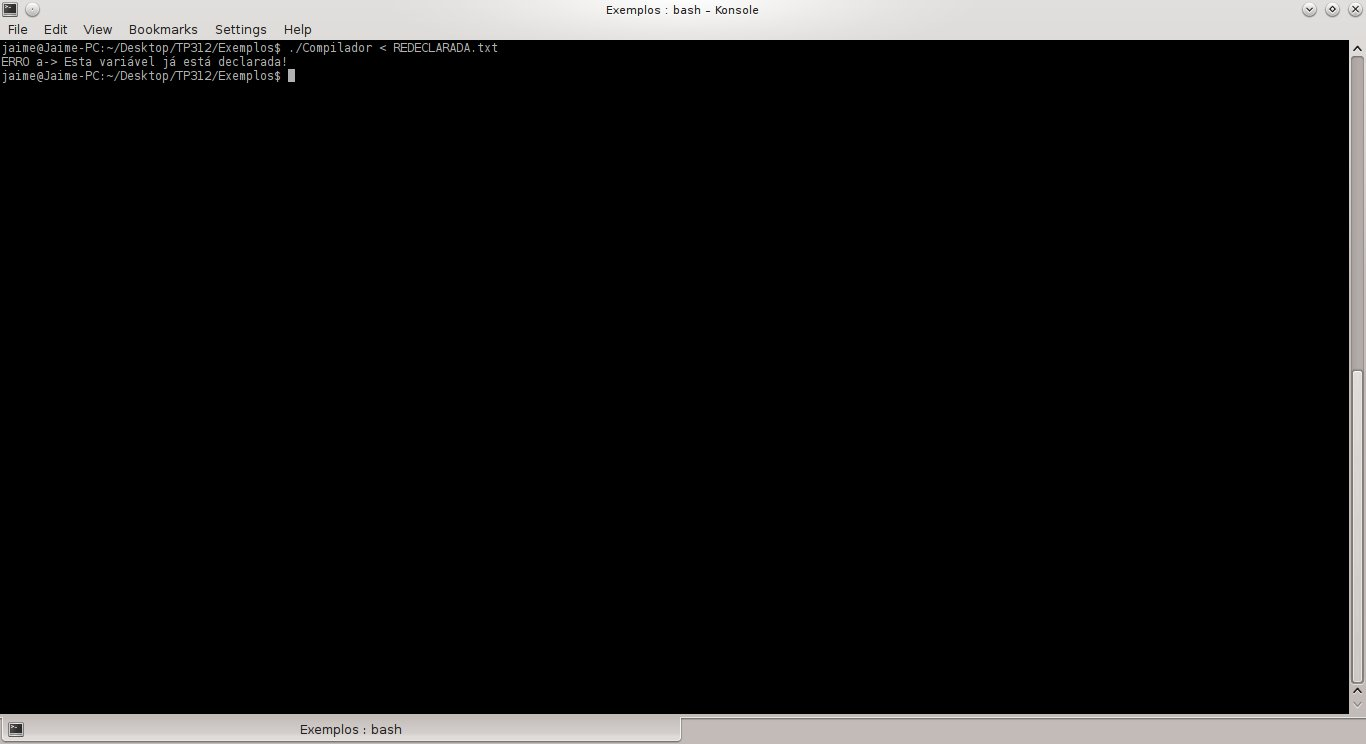
\includegraphics[width=\linewidth]{Redeclarada.jpg}

\section{Condicionais e Ciclos}
Neste exemplo vamos testar ciclos e condições "IF THEN ELSE". A variável "c" é inicializada a TRUE por isso no primeiro IF vamos derivar pelo "Tasks" do THEN one vai ser escrita uma string com o valor do "a" durante o ciclo e o valor de "a" vai ser decrementado. De seguida, vamos executar outro IF mas desta vez como "d" foi inicializado como FALSE vai derivar pelo ELSE que irá entrar num ciclo que irá printar o valor de "b" e incrementar o mesmo.
\subsection{Input:}
\VerbatimInput{1IFUNTIL.txt}
Podemos ver na vm que o valor de "a" é corretamente escrito ao longo do ciclo o que indica que está a ser decrementado, e o mesmo se verifica para o "b" que vai ser incrementado.
\subsection{Output:}

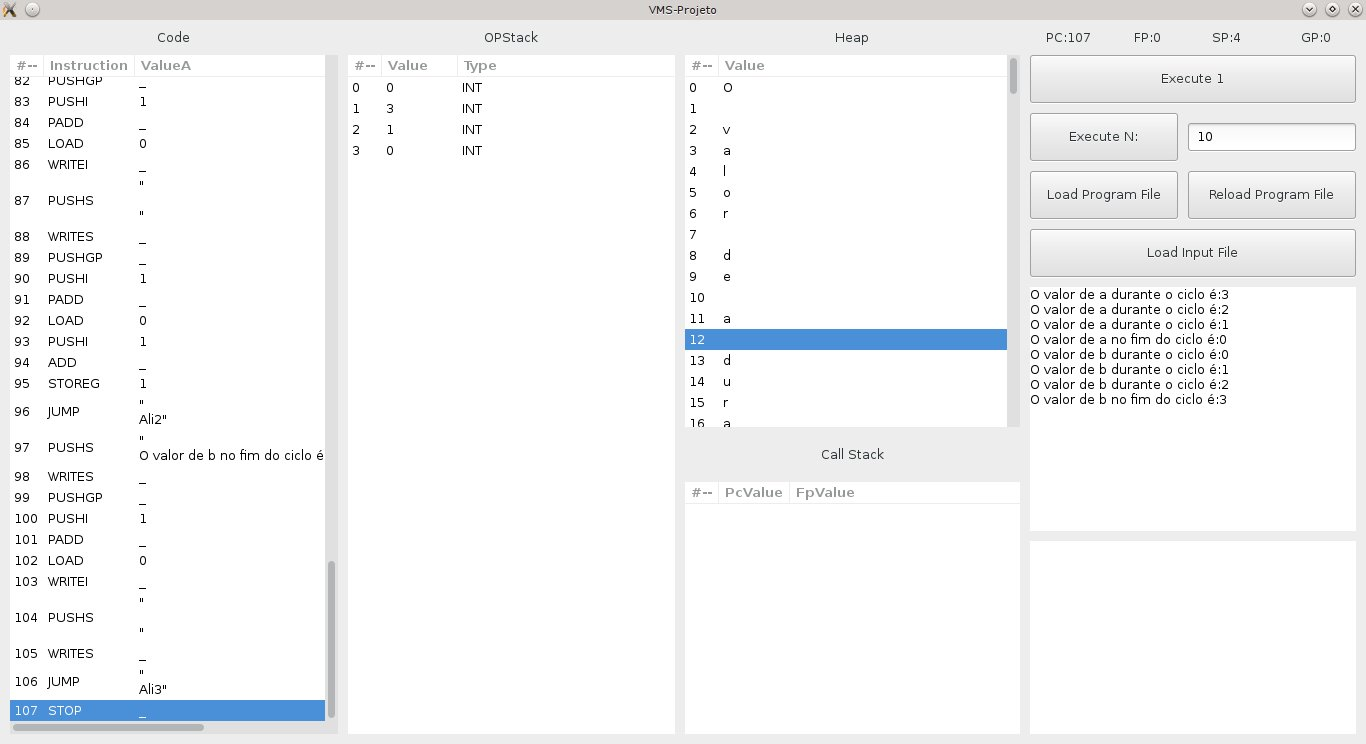
\includegraphics[width=\linewidth]{IfUntilReadWrite.jpg}


\section{Leitura de variáveis}
Este exemplo serve para demonstrar a capacidade de leitura de variáveis tanto reais como inteiras. Começa-se por fazer a escrita da concatenação de duas strings e a leitura de uma variável booleana. Dependendo do valor desta variável, o ramo do if a ser precorrido vai encontrar uma leitura de um real ou inteiro.
\subsection{Input:}
\VerbatimInput{READ.txt}

Neste caso o "a" foi lido como FALSE como é possível ver pelas múltiplas escritas devido ao ciclo.
\textit{Certos simbolos foram substituidos por * devido a conflito no latex.}
\subsection{Output:}

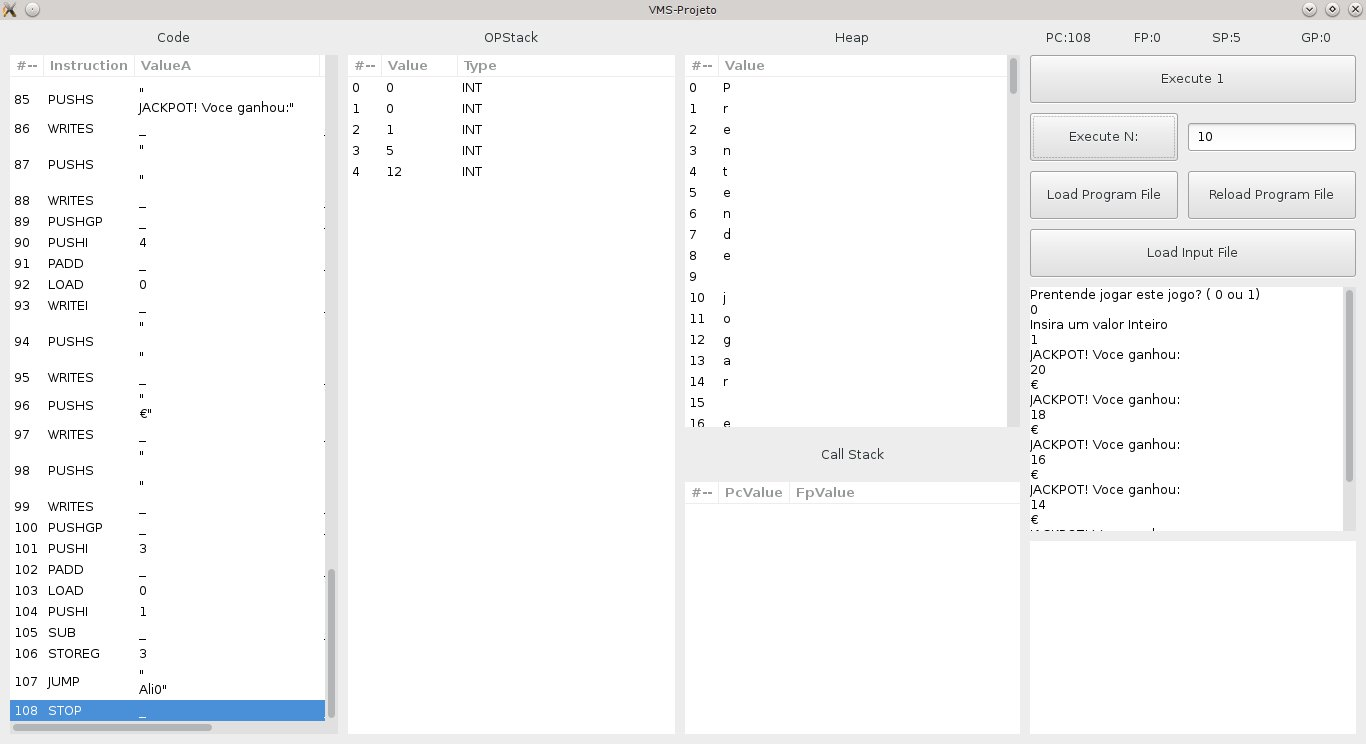
\includegraphics[width=\linewidth]{reads.jpg}

\chapter{Conclusão}
Através deste trabalho, conseguimos entender a utilidade e importância de ferramentas com a capacidade de interpretação de Gramáticas Independentes de contexto na análise léxica.\\
Com o uso destas ferramentas obtemos uma linguagem de programação bastante simples, mas entendemos a potencialidade de aplicação destas no mundo real.\\
Em termos de desafios, o principal foi a distinção entre variáveis Inteiras e Reais de modo a enviar a instrução correta para a Máquina Virtual. Daqui surge a principal limitação da nossa implementação, que assenta no uso de expressões regulares distintas para a diferenciação entre Reais e Inteiros, devido à existência de derivações diferentes para ambos os tipos de variáveis em determinadas operações.\\
Concluindo, somos da opinião que este trabalho foi razoavelmente bem conseguido, tendo em conta as limitações mencionadas, uma vez que conseguimos obter resultados satisfatórios dos diferentes testes que fizemos.

\appendix
\chapter{Código Bison:}
\VerbatimInput{ygram.y}
\chapter{Código Flex:}
\textit{Este ficheiro nao é o utilizado na compilação, uma das linhas teve que ser ocultada devido a conflito com latex, verificar proc.l em anexo.}
\VerbatimInput{procc.l}
\chapter{Biblioteca em C:}
\VerbatimInput{aux.h}




\end{document}
